% **************************************************
% Document Class Definition
% **************************************************
\documentclass[%
    paper=A4,               % paper size --> A4 is default in Germany
    twoside=true,           % onesite or twoside printing
    openright,              % doublepage cleaning ends up right side
    parskip=full,           % spacing value / method for paragraphs
    chapterprefix=true,     % prefix for chapter marks
    11pt,                   % font size
    headings=normal,        % size of headings
    bibliography=totoc,     % include bib in toc
    listof=totoc,           % include listof entries in toc
    titlepage=on,           % own page for each title page
    captions=tableabove,    % display table captions above the float env
    chapterprefix=false,    % do not display a prefix for chapters
    appendixprefix=false,   % but display a prefix for appendix chapter
    draft=false,            % value for draft version
]{scrreprt}%


% **************************************************
% Setup YOUR thesis document in this file !
% **************************************************
% !TEX root = main.tex


% **************************************************
% Files' Character Encoding
% **************************************************
\PassOptionsToPackage{utf8}{inputenc}
\usepackage{inputenc}


% **************************************************
% Information and Commands for Reuse
% **************************************************
\newcommand{\thesisTitle}{Simplifying NeRF: Creating an Intuitive Web-Based 3D Scene Interface}
\newcommand{\thesisName}{Eduard Aurelius von Briesen Brandenburg Neumark}
\newcommand{\thesisSubject}{Master`s Thesis}
\newcommand{\thesisDate}{\today}
\newcommand{\thesisVersion}{0.1}

% \newcommand{\thesisFirstReviewer}{Eyke H{\"u}llermeier}
% \newcommand{\thesisFirstReviewerUniversity}{\protect{LMU Munich}}
% \newcommand{\thesisFirstReviewerDepartment}{Institute of Informatics}

\newcommand{\thesisFirstSupervisor}{Prof. Dr. Sylvia Rothe}
\newcommand{\thesisSecondSupervisor}{Christoph Johannes Weber}

\newcommand{\thesisUniversity}{LMU Munich}
\newcommand{\thesisUniversityDepartment}{Department of Mathematics, Informatics and Statistics}
\newcommand{\thesisUniversityInstitute}{Institute of Informatics}
\newcommand{\thesisUniversityGroup}{}
\newcommand{\thesisUniversityCity}{Munich}
\newcommand{\thesisUniversityStreetAddress}{Akademiestra\ss e 7}
\newcommand{\thesisUniversityPostalCode}{80799 Munich}


% **************************************************
% Debug LaTeX Information
% **************************************************
%\listfiles

% **************************************************
% Load and Configure Packages
% **************************************************
\usepackage[english]{babel} % babel system, adjust the language of the content
\PassOptionsToPackage{% setup clean thesis style
    figuresep=colon,%
    hangfigurecaption=false,%
    hangsection=true,%
    hangsubsection=true,%
    sansserif=false,%
    configurelistings=true,%
    colorize=full,%
    colortheme=lmuaiml,%
    configurebiblatex=true,%
    bibsys=bibtex,%
    bibfile=bib-refs,%
    bibstyle=numeric,%
    bibsorting=nty,%
}{cleanthesis}
\usepackage{cleanthesis}

\usepackage{mathtools}

\hypersetup{% setup the hyperref-package options
    pdftitle={\thesisTitle},    %   - title (PDF meta)
    pdfsubject={\thesisSubject},%   - subject (PDF meta)
    pdfauthor={\thesisName},    %   - author (PDF meta)
    plainpages=false,           %   -
    colorlinks=false,           %   - colorize links?
    pdfborder={0 0 0},          %   -
    breaklinks=true,            %   - allow line break inside links
    bookmarksnumbered=true,     %
    bookmarksopen=true          %
}

% **************************************************
% Other Packages
% **************************************************
\usepackage{scrhack}
\usepackage{lipsum}
\usepackage{tikz}% do not disable this package

\usetikzlibrary{backgrounds,calc}

\usepackage{pgf-pie}
\usepackage{tabularx}
\usepackage{listings}
\usepackage{subcaption}
\usepackage{todonotes}
\usepackage{wrapfig}
\usepackage{pgfplots}
\pgfplotsset{compat=1.17}


\usepackage[top=3cm,left=3cm,right=3cm,bottom=4cm]{geometry}

\lstdefinelanguage{JavaScript}{
  morekeywords=[1]{break, continue, delete, else, for, function, if, in,
    new, return, this, typeof, var, void, while, with},
  % Literals, primitive types, and reference types.
  morekeywords=[2]{false, null, true, boolean, number, undefined, string,
    Array, Boolean, Date, Math, Number, String, Object},
  % Built-ins.
  morekeywords=[3]{eval, parseInt, parseFloat, escape, unescape},
  sensitive,
  morecomment=[s]{/*}{*/},
  morecomment=[l]//,
  morecomment=[s]{/**}{*/}, % JavaDoc style comments
  morestring=[b]',
  morestring=[b]"
}[keywords, comments, strings]

\lstalias[]{ES6}[ECMAScript2015]{JavaScript}

\lstdefinelanguage[ECMAScript2015]{JavaScript}[]{JavaScript}{
  morekeywords=[1]{await, async, case, catch, class, const, default, do,
    enum, export, extends, finally, from, implements, import, instanceof,
    let, static, super, switch, throw, try},
  morestring=[b]` % Interpolation strings.
}

% Requires package: color.
\definecolor{mediumgray}{rgb}{0.3, 0.4, 0.4}
\definecolor{mediumblue}{rgb}{0.0, 0.0, 0.8}
\definecolor{forestgreen}{rgb}{0.13, 0.55, 0.13}
\definecolor{darkviolet}{rgb}{0.58, 0.0, 0.83}
\definecolor{royalblue}{rgb}{0.25, 0.41, 0.88}
\definecolor{crimson}{rgb}{0.86, 0.8, 0.24}

\lstdefinestyle{JSES6Base}{
  % backgroundcolor=\color{white},
  basicstyle=\ttfamily,
  breakatwhitespace=false,
  breaklines=false,
  captionpos=b,
  columns=fullflexible,
  commentstyle=\color{mediumgray}\upshape,
  emph={},
  emphstyle=\color{crimson},
  extendedchars=true,  % requires inputenc
  fontadjust=true,
  % frame=single,
  % identifierstyle=\color{black},
  keepspaces=true,
  keywordstyle=\color{mediumblue},
  keywordstyle={[2]\color{darkviolet}},
  keywordstyle={[3]\color{royalblue}},
  numbers=left,
  % numbersep=15pt,
  % numberstyle=\tiny\color{black},
  % rulecolor=\color{black},
  showlines=true,
  showspaces=false,
  showstringspaces=false,
  showtabs=false,
  stringstyle=\color{forestgreen},
  tabsize=2,
  title=\lstname,
  upquote=true  % requires textcomp
}

\lstdefinestyle{JavaScript}{
  language=JavaScript,
  style=JSES6Base
}
\lstdefinestyle{ES6}{
  language=ES6,
  style=JSES6Base
}





% **************************************************
% Document CONTENT
% **************************************************
\begin{document}

% --------------------------
% rename document parts
% --------------------------
%\renewcaptionname{ngerman}{\figurename}{Abb.}
%\renewcaptionname{ngerman}{\tablename}{Tab.}
\renewcaptionname{english}{\figurename}{Fig.}
\renewcaptionname{english}{\tablename}{Tab.}

% --------------------------
% Front matter
% --------------------------
\pagenumbering{roman}			% roman page numbing (invisible for empty page style)
\pagestyle{empty}				% no header or footers
% !TEX root = ../main.tex
%
% ------------------------------------  --> cover title page
\begin{titlepage}
	\pdfbookmark[0]{Cover}{Cover}
	\flushright
	\hfill
	\vfill
	{\LARGE\thesisTitle \par}
	\rule[5pt]{\textwidth}{.4pt} \par
	{\Large\thesisName}
	\vfill
	\textit{\large\thesisDate} \\
	Version: \thesisVersion
\end{titlepage}


% ------------------------------------  --> main title page
\begin{titlepage}
	\pdfbookmark[0]{Titlepage}{Titlepage}
	\tgherosfont
	
	
	\begin{figure}
	\begin{minipage}[t]{8.5cm}		
	
\includegraphics[height=1.8cm,width=3.6cm]{gfx/lmulogo.pdf}\\
	\textsf{\small{Department of Mathematics,  \\ Informatics and Statistics, \\
		\thesisUniversityInstitute
%		\textsf{\small{
%		\hspace*{1.3cm}Warburger Straße 100 \\
%		\hspace*{1.3cm}33098 Paderborn
		}}
	\end{minipage}
	\hfill
	\begin{minipage}[t]{4.7cm}
	
\includegraphics[height=1.5cm]{gfx/hff-logo-small.jpeg}\\
	\textsf{\small{Munich Film School, \\ Chair for AI}}
	\end{minipage}
	\end{figure}
	
	\centering
	%\textsf{\thesisUniversityDepartment} \\
	%\textsf{\thesisUniversityInstitute} \\
	%\textsf{\thesisUniversityGroup} \\

	\vfill
	{\large \thesisSubject} \\[5mm]
	{\LARGE \color{ctcolortitle}\textbf{\thesisTitle} \\[10mm]}
	{\Large \thesisName} \\

	\vfill
	% \begin{minipage}[t]{.27\textwidth}
	% 	\raggedleft
	% 	\textit{Reviewer}
	% \end{minipage}
	% \hspace*{15pt}
	% \begin{minipage}[t]{.65\textwidth}
	% 	{\Large \thesisFirstReviewer} \\
	%   	{\small \thesisFirstReviewerDepartment} \\[-1mm]
	% 	{\small \thesisFirstReviewerUniversity}
	% \end{minipage} \\[10mm]
	\begin{minipage}[t]{.27\textwidth}
		\raggedleft
		\textit{Supervisors}
	\end{minipage}
	\hspace*{15pt}
	\begin{minipage}[t]{.65\textwidth}
		\thesisFirstSupervisor\ and \thesisSecondSupervisor
	\end{minipage} \\[10mm]

	\thesisDate\\
	
	\begin{tikzpicture}[remember picture,overlay]
		\begin{pgfonlayer}{background}
			\node[anchor=south east,outer sep=0pt,inner sep=0pt] at ($(current page.south east) +(-0in,0in)$) {
\includegraphics[trim=0 55 100 00,clip,width=0.2\paperheight,height=0.25\paperheight]{gfx/siegel.pdf}};
		\end{pgfonlayer}
	\end{tikzpicture}

\end{titlepage}


% ------------------------------------  --> lower title back for single page layout




\hfill
\vfill
{
	\small
	\textbf{\thesisName} \\
	\textit{\thesisTitle} \\
	\thesisSubject, \thesisDate \\
	% Reviewers: \thesisFirstReviewer\ \\
	Supervisors: \thesisFirstSupervisor\ and \thesisSecondSupervisor \\[1.5em]
	\textbf{\thesisUniversity} \\
	\thesisUniversityDepartment \\
	\thesisUniversityInstitute \\
	\textit{\thesisUniversityGroup} \\
	\thesisUniversityStreetAddress \\
	\thesisUniversityPostalCode\ 
} 
		% INCLUDE: all titlepages
\cleardoublepage

\pagestyle{plain}				% display just page numbers
% !TEX root = ../main.tex
%
\pdfbookmark[0]{Abstract}{Abstract}
\chapter*{Abstract}
\label{sec:abstract}
\vspace*{-10mm}

\blindtext

\vspace*{20mm}

{\usekomafont{chapter}Abstract (different language)}\label{sec:abstract-diff} \\

\lipsum[1]
		% INCLUDE: the abstracts (english and german)
\cleardoublepage
%
% !TEX root = ../main.tex
%
\pdfbookmark[0]{Acknowledgement}{Acknowledgement}
\chapter*{Acknowledgement}
\label{sec:acknowledgement}
\vspace*{-10mm}

 % INCLUDE: acknowledgement
\cleardoublepage
%
\currentpdfbookmark{\contentsname}{toc}
\setcounter{tocdepth}{2}		% define depth of toc
\tableofcontents				% display table of contents
\cleardoublepage

% --------------------------
% Body matter
% --------------------------
\pagenumbering{arabic}			% arabic page numbering
\setcounter{page}{1}			% set page counter
\pagestyle{scrheadings} 	% fancy header and footer

% !TEX root = ../main.tex
%
\chapter{Introduction}
\label{sec:intro}

% \section{Background}
% \label{sec:intro:background}

Neural Radiance Fields (NeRF) have emerged as a transformative technology in 3D scene modeling and rendering, offering unprecedented realism and detail. 
This advancement has significantly impacted various applications, from virtual reality to cultural heritage preservation. 

Two prominent NeRF frameworks with user interfaces, namely Instant NGP \cite{muller_instant_2022} and Nerfstudio \cite{tancik_nerfstudio_2023}, have emerged as leaders in enabling users to explore and manipulate 3D scenes. 
These frameworks offer features such as real-time scene rendering, adjustable training parameters, and the creation of camera trajectories for video rendering.

Additionally, several innovative projects have expanded the NeRF landscape. Notably, CLIP-NeRF \cite{wang_clip-nerf_2022}, Instruct-NeRF2NeRF \cite{haque_instruct-nerf2nerf_2023}, Text2LIVE \cite{bar-tal_text2live_2022}, and SINE \cite{bao_sine_2023} have introduced text-based editing approaches, broadening the possibilities for manipulating NeRF models. PaletteNeRF \cite{wu_palettenerf_2022} focuses on color editing, while NeRF-Editing \cite{yuan_nerf-editing_2022} enables mesh editing. 

Despite these advancements, the technical complexity of these frameworks frequently acts as a barrier to broader accessibility, indicating a need for improvements in user experience. 
These interfaces usually require a high degree of technical knowledge, as they are intended to supplement, rather than substitute, command-line interfaces.
For activities like video data preprocessing, model training, and output rendering, users are required to navigate through terminal-based processes.

This complexity not only limits the potential user base to individuals with technical expertise but also hinders the creative and innovative application of NeRF technology across broader fields. 
Consequently, there exists a critical need to enhance the user experience and develop solutions that simplify the interaction with NeRF frameworks, making them more approachable and usable for a diverse range of users beyond the realm of technical specialists.


\section*{Research Objectives}
\label{sec:intro:objectives}

The research objectives of this study are as follows:

\begin{enumerate}
    \item \textbf{Exploration of NeRF Interaction Capabilities}: This study aims to explore the existing interaction capabilities within NeRF frameworks comprehensively. It involves an analysis of the current state of NeRF interfaces and an investigation into user engagement, visualizations, and manipulation of NeRF scenes.

    \item \textbf{Development of a Web-Based User Interface}: Building on insights gained from the exploration phase, the primary objective is to design and implement a user-friendly web-based interface for NeRF.

    \item \textbf{Streamlined NeRF Creation and Manipulation}: The central goal is to simplify the process of NeRF creation and manipulation, eliminating the need for users to deal with complex command-line interfaces or extensive local setup. The web-based interface will provide an intuitive and efficient user experience.

    \item \textbf{Integration of Diverse Editing Plugins}: To enhance the creative potential of NeRF, various editing plugins will be integrated into the web-based interface. The objective is to expand the functionality and versatility of the NeRF framework.
\end{enumerate}

The research aims to advance NeRF frameworks' capabilities and accessibility, making them accessible to a broader audience and fostering innovation in 3D scene modeling and rendering.


\section*{Research Question}
\label{sec:intro:question}

This research is guided by the following questions:

\begin{enumerate}
    \item \textbf{Enhancing NeRF Frameworks:} How can a web-based interface improve the user experience and accessibility of NeRF frameworks, and what impact will these enhancements have on user-friendly NeRF creation and manipulation?

    \item \textbf{Overcoming Technical Challenges:} What technical challenges and limitations are associated with current NeRF frameworks and interfaces, and how can innovative design and technology choices in a web-based interface overcome these challenges?

    \item \textbf{Innovative Editing Integration:} How can novel editing approaches be seamlessly integrated into a web-based NeRF interface to enhance creativity and usability, and how do these methods compare with traditional NeRF editing techniques?
\end{enumerate}

\section*{Scope of the Study}
\label{sec:intro:scope}
This research focuses on the development and evaluation of a web-based interface for NeRF, aiming to improve its accessibility and usability. 
The study will concentrate on interface design, user interaction, and the integration of editing functionalities, without delving into the underlying algorithms of NeRF technology itself. 
It is delimited by its emphasis on interface design over algorithmic advancements in NeRF processing.

\section*{Significance of the Study}
\label{sec:intro:significance}
By addressing the usability challenges of current NeRF frameworks, this research aims to make 3D scene modeling more accessible, fostering innovation and broadening the application of this technology across various fields. 
The development of a web-based interface could significantly lower the entry barrier to NeRF, enabling artists, designers, and educators to leverage this technology without requiring deep technical expertise.

% TODO ?
% \section*{Structure of the Thesis}
% \label{sec:intro:structure}
% The thesis is structured as follows:

% \textbf{Chapter 2: Related Works} reviews existing NeRF frameworks, user interfaces, and editing tools, providing context for this research.
% \textbf{Chapter 3: Methodology} details the research methods employed in developing and evaluating the web-based interface.
% Subsequent chapters will cover the development process, evaluation results, discussion, and conclusions, culminating in recommendations for future research.   % INCLUDE: introduction
% !TEX root = ../main.tex
%
\chapter{Related Work}
\label{sec:related}

\section{Instant NGP}

Instant Neural Graphics Primitives (Instant NGP) \cite{muller_instant_2022}, developed by NVIDIA, utilizes a multiresolution hash encoding that simplifies models while maintaining high performance and quality.
Its graphical user interface (GUI) plays a crucial role in enhancing accessibility and functionality, making it an important advancement in neural graphics technology.

\cleanparagraph{Simplified User Interaction}
The user interface of Instant NGP facilitates training and visualization of NeRFs \fref{fig:instant-ngp}.
The user is able to interactively explore 3D scenes in real-time and adjust parameters in order to achieve the desired results.

\begin{figure}[h!]
  \centering
  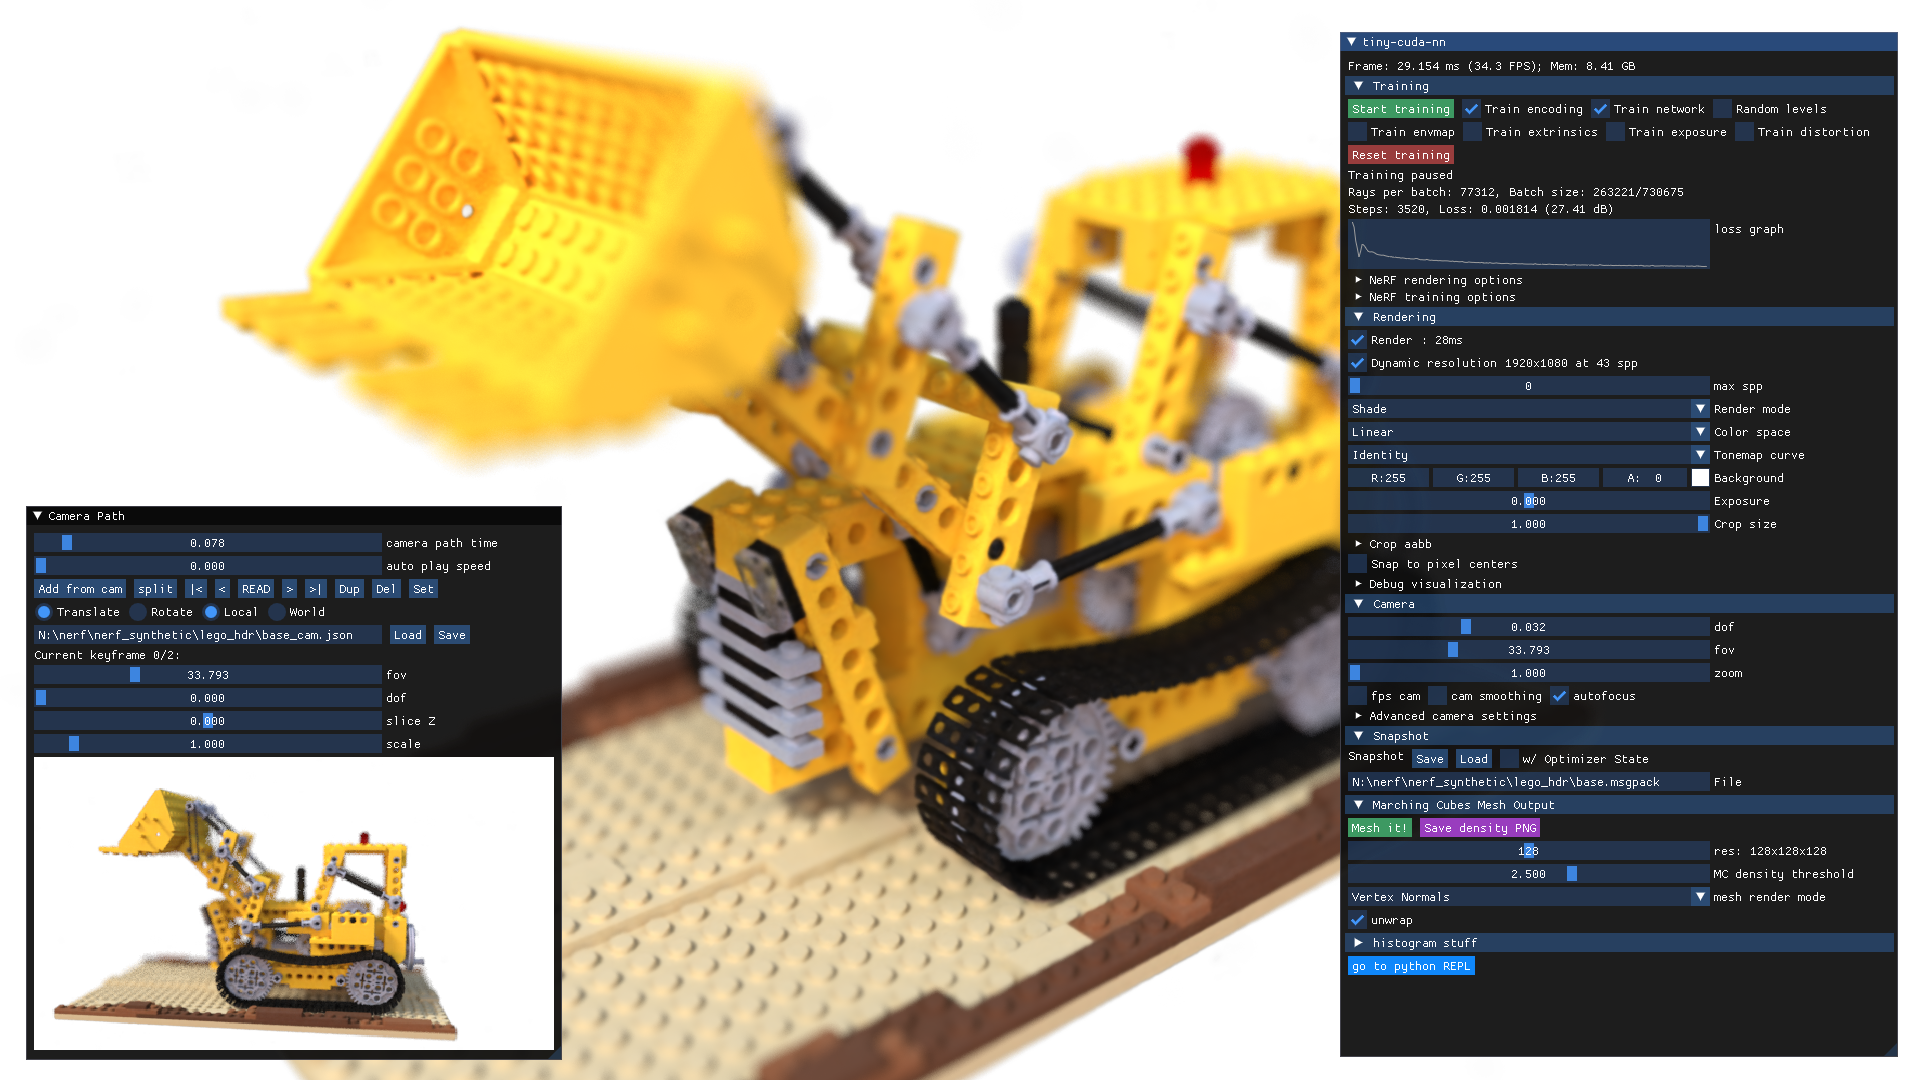
\includegraphics[width=\textwidth]{figures/realted-instant-ngp.png}
  \caption{Instant NGP's GUI rendering a NeRF scene, showing the 3D scene, camera path editor, and training parameters.
   \cite{muller_instant_2022}.}
  \label{fig:instant-ngp}
\end{figure}

\cleanparagraph{VR Mode}
The virtual reality (VR) mode of Instant NGP enhances user interaction by enabling immersive exploration of 3D environments in real-time.
This feature is especially beneficial for professionals like architects and game developers, who can benefit from experiencing their virtual spaces as if they were real.

\cleanparagraph{Camera Path Editor}
Instant NGP's camera path editor allows users to intuitively create and adjust camera trajectories, enhancing the creation of animations.
This tool is essential to professionals in visualization and animation, providing precise control over camera movements for detailed and smooth outputs.

\cleanparagraph{Limitations}
Despite advancements, Instant NGP's technical complexity and reliance on command-line interfaces for key operations remain significant barriers.
These aspects limit its accessibility to those with specific technical skills and deter broader creative applications.
The user experience still requires technical expertise, underscoring the need for more intuitive interfaces that simplify interaction and expand the user base beyond that of technical specialists.

\section{Nerfstudio}
\label{sec:related:nerfstudio}

Nerfstudio \cite{tancik_nerfstudio_2023} represents a significant advance in the accessibility of Neural Radiance Fields to non-technical users.
Its design focuses on modularity, ease of use, and integration capabilities, which are crucial for practical applications and academic research.

\cleanparagraph{Modularity}
Nerfstudio is built on a modular framework that allows users to easily customize and extend their NeRF implementations.
This modularity enables the use of a variety of input data formats, making it versatile for different real-world scenarios and setting it apart from Instant NGP.
A wide range of existing methods are already well integrated into Nerfstudio, including Instant-GPT \cite{muller_instant_2022}, their own Nerfacto \cite{noauthor_nerfacto_nodate} method that combines various existing techniques, and several of the previously mentioned extensions \cite{haque_instruct-nerf2nerf_2023,jan-niklas_dihlmann_signerf_2024}.

\cleanparagraph{Real-Time Web Viewer}
One of the standout features of Nerfstudio is its real-time web viewer, which enables visualization of NeRF training progress and outputs directly through a web browser \fref{fig:nerfstudio-viewer}.
This eliminates the need for high-end local GPU setups, such as in the case of Instant NGP, through remote sessions, broadening the tool's accessibility \cite{noauthor_nerfstudio-projectviser_2024}.

\begin{figure}[h!]
  \centering
  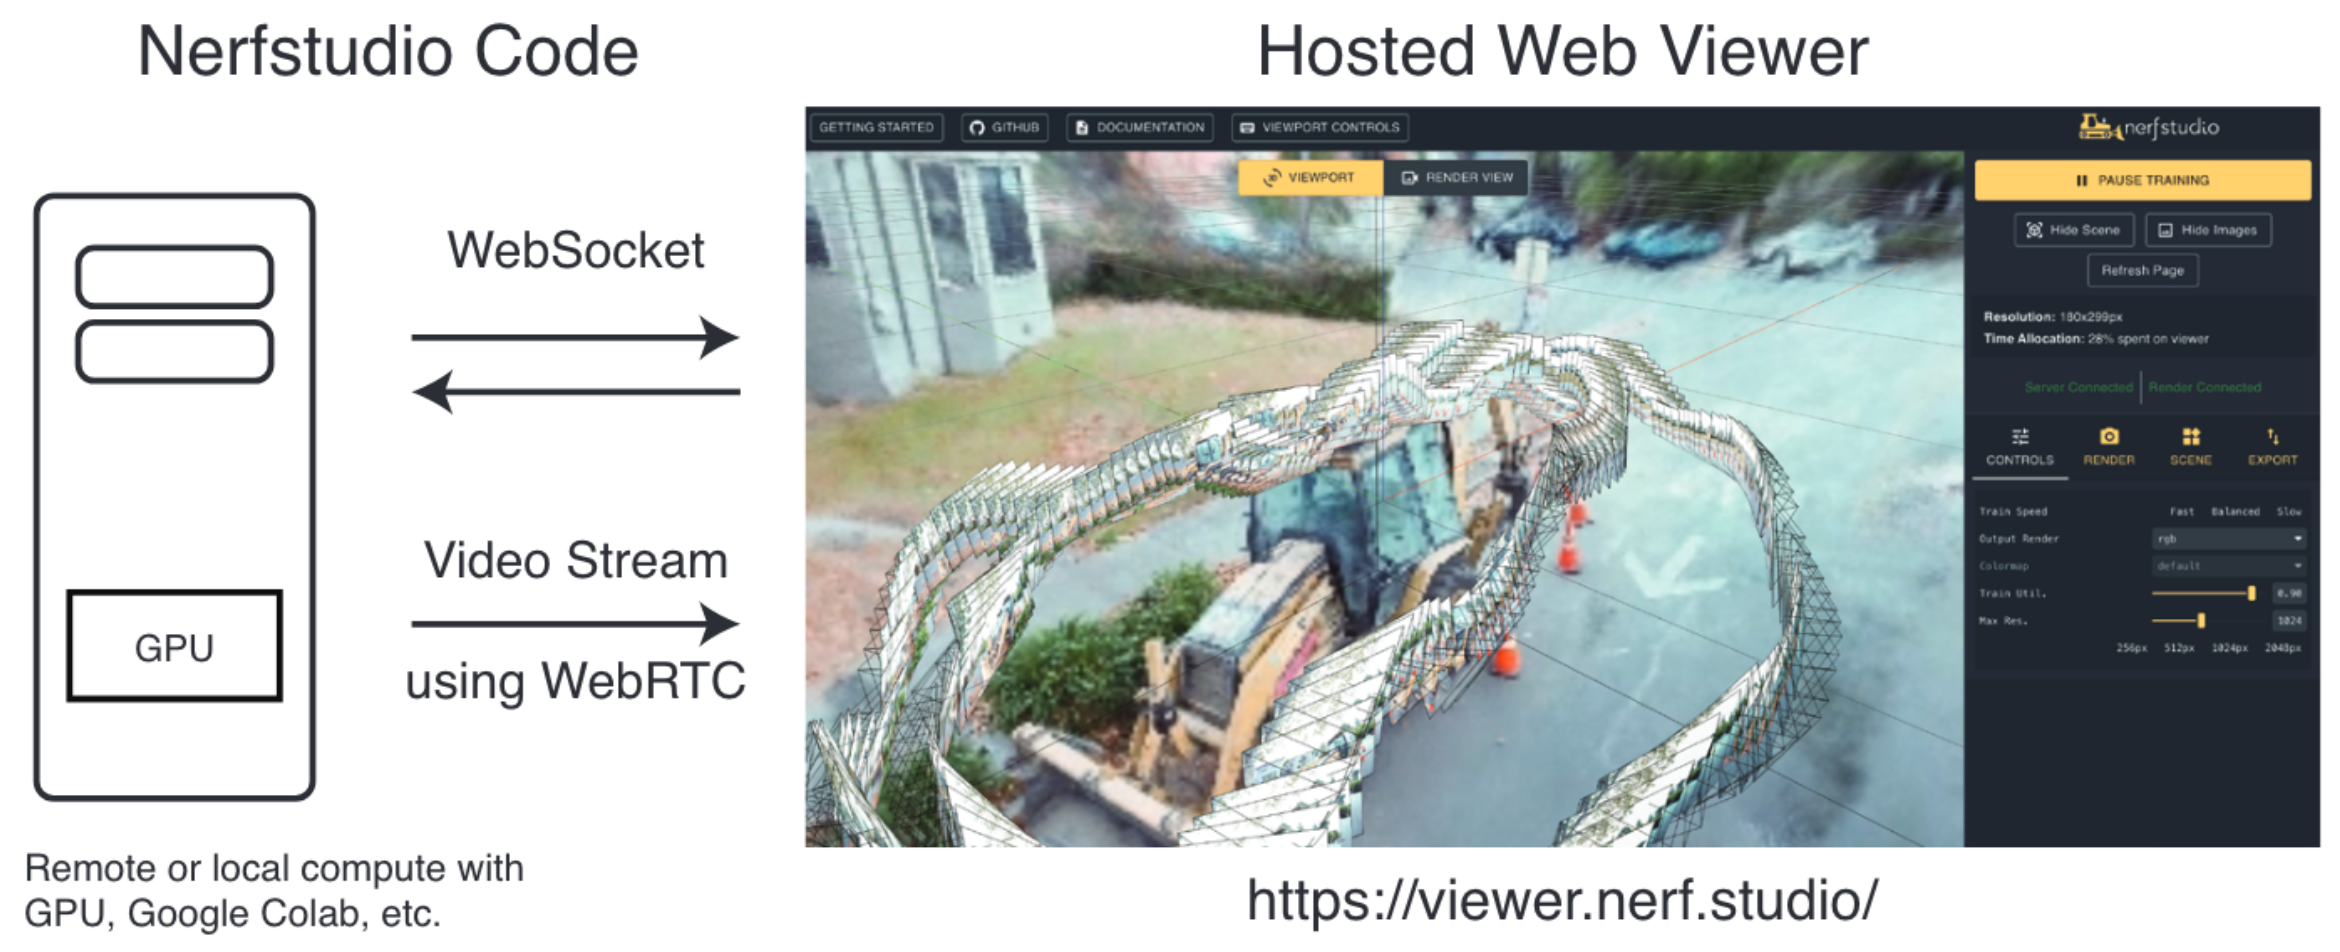
\includegraphics[width=\textwidth]{figures/related-nerfstudio-viewer.png}
  \caption{Nerfstudio's web viewer connected to a remote server running the training \cite{tancik_nerfstudio_2023}.}
  \label{fig:nerfstudio-viewer}
\end{figure}

\cleanparagraph{Flexibility of Data Handling}
Nerfstudio simplifies importing and exporting data, supporting a wide range of formats to accommodate various use cases.
Users can easily import images and videos, including data from mobile capture apps such as Polycam \cite{noauthor_polycam_nodate} and Record3D \cite{noauthor_record3d_nodate}.
Additionally, the framework supports exporting results in various formats such as videos, point clouds, and meshes.
This flexibility allows users to integrate NeRF outputs into diverse creative and technical applications.

\cleanparagraph{Community and Open-Source Contribution}
As an open-source project, Nerfstudio encourages community-driven development and continuous improvement, facilitating updates that keep pace with the latest research and technological advances.
This openness also allows users to adapt the tool to their specific needs.

\cleanparagraph{Limitations}
Nerfstudio is a welcome advancement improving on much of the features of Instant NGP.
However, it still requires a certain level of technical knowledge to operate effectively, limiting accessibility to non-technical users.
The tool's primary interactions are still command-line based, which presents a barrier to users who may prefer more intuitive graphical interfaces.

\section{Luma AI}
\label{sec:related:luma}

Luma AI \cite{noauthor_luma_nodate} is making Neural Radiance Fields accessible to non-technical users in a commercial space.
This platform leverages augmented reality (AR) to guide users through the capture process, greatly simplifying the creation of NeRFs from everyday smartphones.

\cleanparagraph{Guided Capture Process}
Luma AI utilizes AR to assist users in capturing images from optimal angles and distances, ensuring that the collected data is suitable for NeRF generation.
This guided process reduces the complexities involved in capturing the necessary footage for effective and streamlined NeRF creation.

\cleanparagraph{Cloud-Based NeRF Generation}
Once the footage is captured, it is automatically processed in Luma AI’s cloud-based system to generate a NeRF, requiring no user input for configuration.
This automation not only simplifies the user experience but also makes powerful 3D reconstruction technology readily accessible to a broad audience.

\cleanparagraph{Viewing and Editing}
Created scenes can be viewed directly within the app or through a web browser \fref{fig:luma-viewer}. 
While the editing capabilities are limited, users can make basic adjustments, reshoot parts of the scene, and interact with the generated NeRF in an intuitive manner.
The features here are similar to those offered in Nerfstudio's viewer, but with a more modern user-interface.

\begin{figure}[h!]
  \centering
  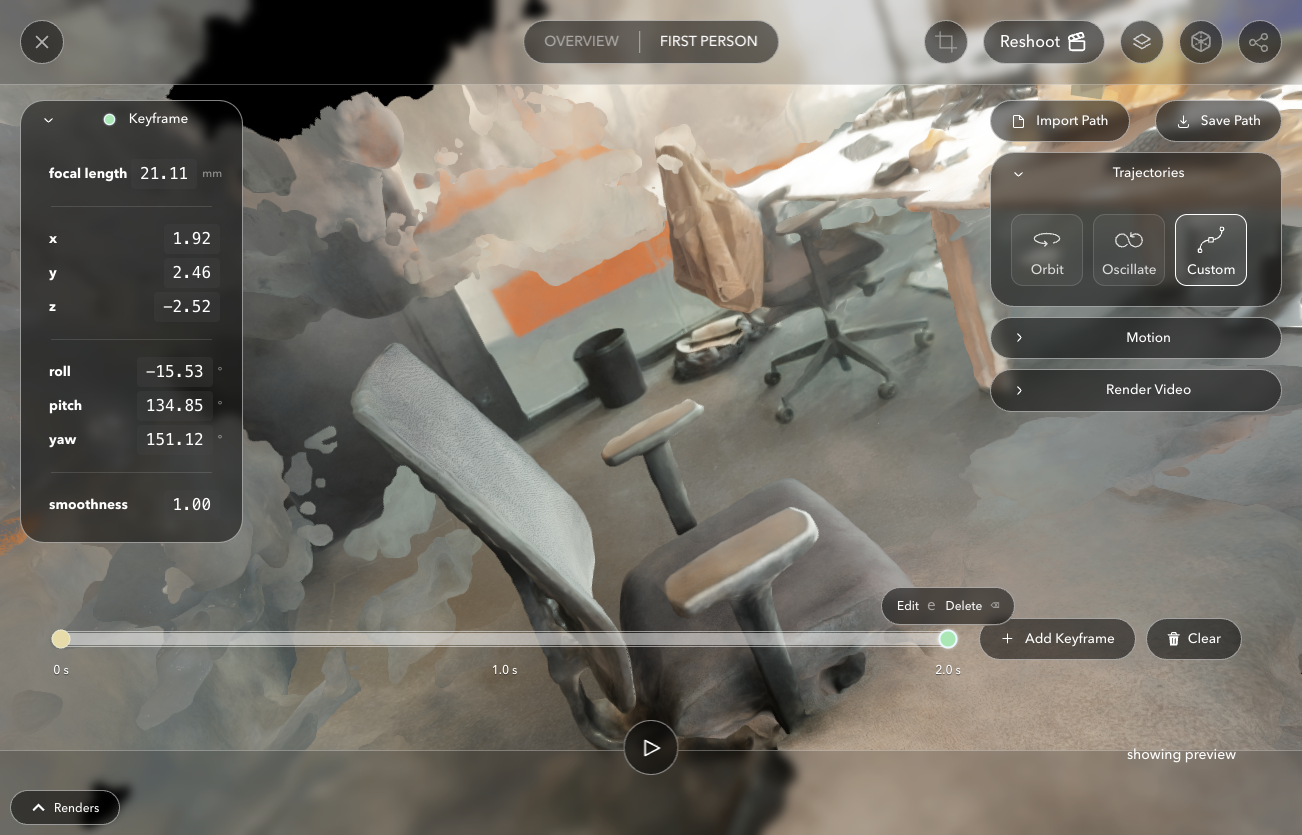
\includegraphics[width=\textwidth]{figures/related-luma.png}
  \caption{Luma AI Web Viewer in the camera path editor.}
  \label{fig:luma-viewer}
\end{figure}

\cleanparagraph{Export Capabilities}
Luma AI offers a variety of export formats for the generated scenes, allowing users to utilize these outputs in different applications or platforms, enhancing the utility of the captured NeRFs.
Additionally, they provide a social platform for the sharing and viewing of NeRFs, fostering a community of users around the technology.

\cleanparagraph{Limitations}
Despite its innovative approach, Luma AI's primary limitation lies in the lack of user control over the NeRF training process.
The automated system is designed to be user-friendly, yet it lacks the capacity to permit adjustments to the training parameters or the refinement of the final model.
This lack of control can result in suboptimal NeRF outputs for users who may require more precise or customized 3D representations.
Additionally, the proprietary nature of Luma AI may be a concern for users who prefer the flexibility and transparency offered by open-source solutions, as it limits the ability to understand and modify the underlying processes.

\section{Volinga Suite}

The Volinga Suite \cite{noauthor_volinga_nodate} aims to integrate Neural Radiance Fields into professional workflows.
It facilitates the adoption of NeRF by leveraging familiar platforms, thereby broadening the accessibility of NeRF to a wider range of users.

\cleanparagraph{Unreal Engine Integration}
Volinga's integration as a plugin for Unreal Engine \cite{noauthor_unreal_nodate} is a core feature that allows users to adopt NeRF seamlessly into existing pipelines \fref{fig:volinga-viewer}.
This integration is valuable for professionals already familiar with Unreal Engine, as it enables them to utilize advanced NeRF functionalities without additional training or significant adjustments to their current workflows.

\begin{figure}[h!]
  \centering
  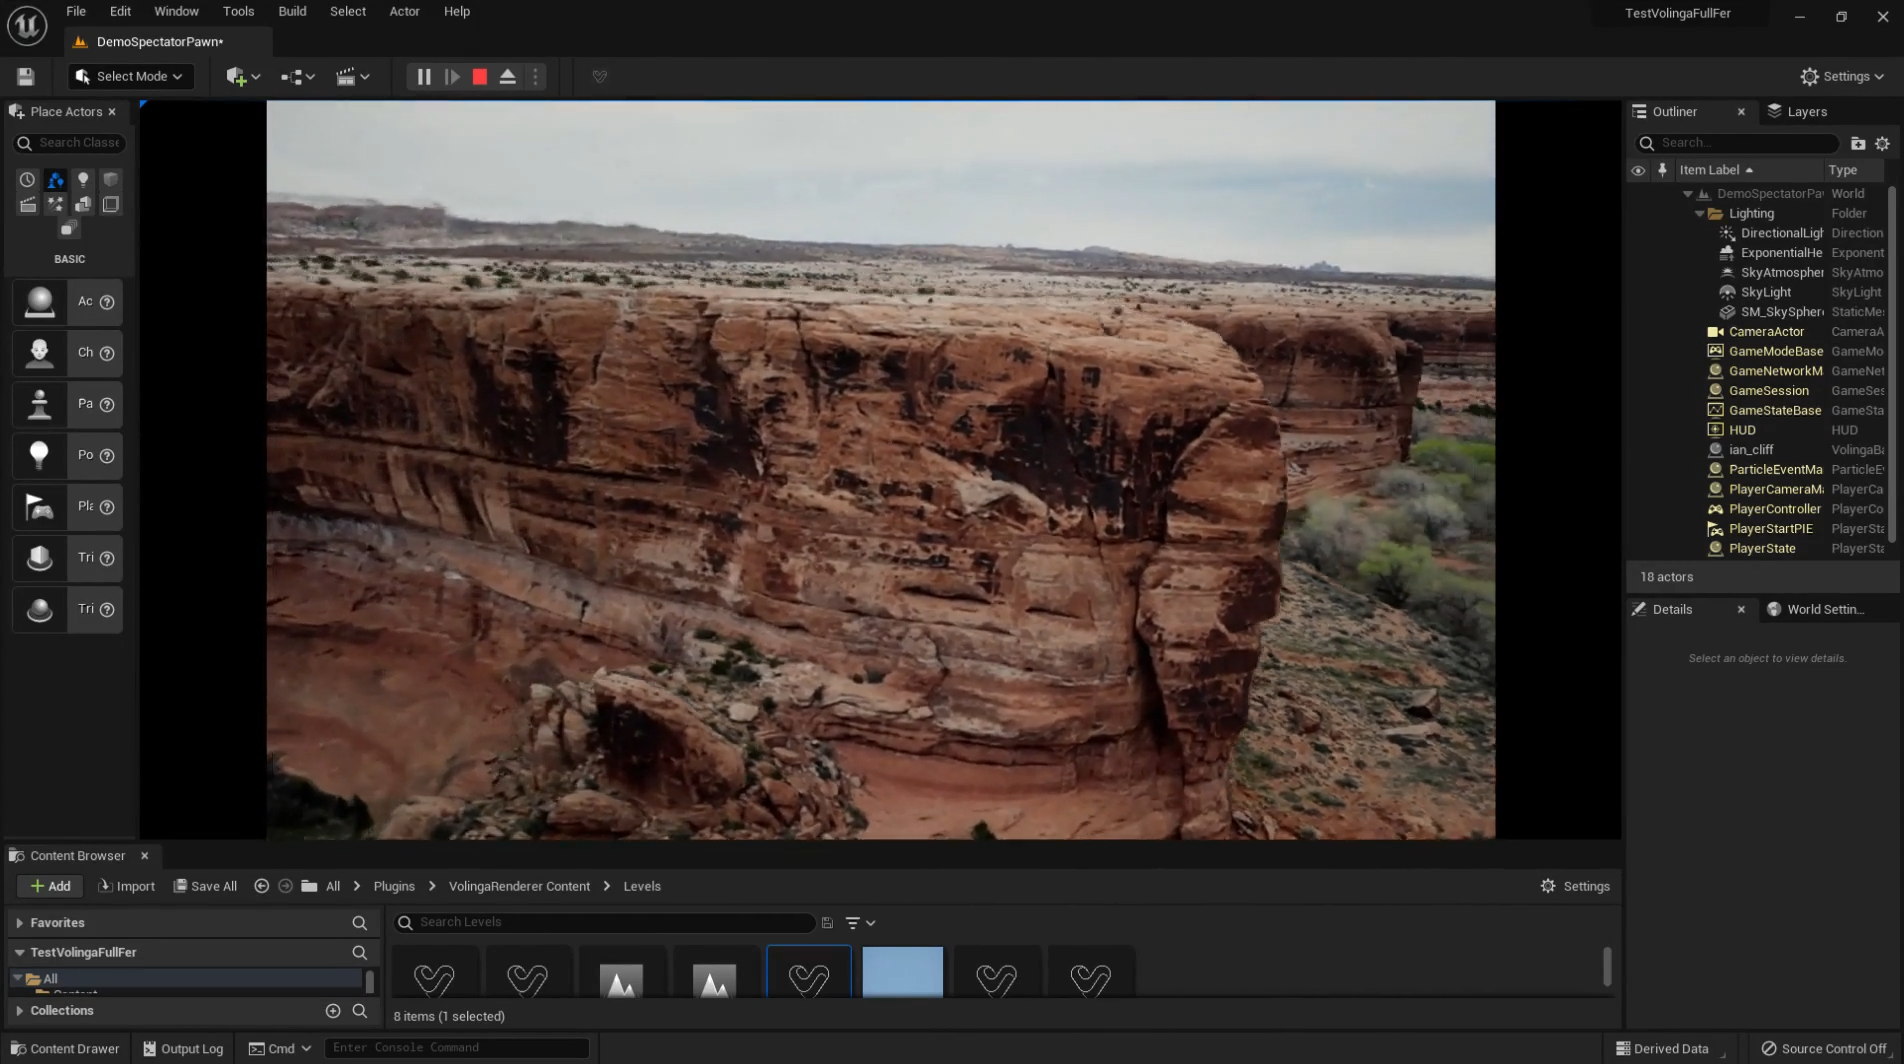
\includegraphics[width=\textwidth]{figures/related-volinga.png}
  \caption{Volinga Suite's integrated viewer in Unreal Engine \cite{noauthor_volinga_nodate}.}
  \label{fig:volinga-viewer}
\end{figure}

\cleanparagraph{Enhanced Control Over Training}
Volinga distinguishes itself from LumaAI by offering enhanced control over the NeRF training process.
Users have the ability to locally adjust numerous parameters, which enables precise tuning of the model's performance to meet specific project requirements.
This level of control is beneficial for projects where the quality of the NeRF output is critical.

\cleanparagraph{Local and Remote Training Capabilities}
The Volinga Creator component supports both local and remote training of NeRF models.
While remote training offers convenience and ease of access, local training provides advanced users with extensive configuration options and the ability to leverage powerful hardware, thereby maximizing the potential of NeRF technology under various usage scenarios.

\cleanparagraph{Limitations}
Volinga Suite's reliance on Unreal Engine for its integrated viewer may limit users who are unfamiliar with or do not wish to use this specific platform.
The web based viewer of Nerfstudio and Luma AI is more accessible in this regard.
Although Volinga is actively contributing to the open-source project Nerfstudio, its proprietary nature may also deter users or organizations that prefer open-source solutions.
   % INCLUDE: related work
% !TEX root = ../main.tex
%
\chapter{Methodology}
\label{sec:methodology}

This research was organized into three sequential phases: initial user research, prototype development, and user testing. 
Each phase was designed to inform and refine the subsequent stages, ensuring a systematic approach to developing a user-friendly NeRF interface. 
This iterative process aimed to align closely with user needs and feedback, fostering a design that is both intuitive and functional.

\section{Initial User Research}
\label{sec:methodology:user-research}

The foundational stage of this research involved conducting a series of in-depth interviews to gather insights into the user experience of NeRF technology. 
The primary objective is to understand the varied challenges, needs, and preferences of users, ranging from novices to experts in NeRF model creation, particularly those with ties to the film industry. 
This exploratory phase is crucial for identifying the key features and improvements necessary for a more accessible and efficient NeRF interface. (see Chapter~\ref{sec:user-research})

\section{Design and Development Process}
\label{sec:methodology:design-development}

The transition from initial user research findings to a functional prototype was a multi-step process focused on capturing user needs and translating them into a tangible design. 
This phase involved the creation of a user flow diagram, site map, wireframes, and a working prototype, each building upon the insights gained from the previous stage. (see Section~\ref{sec:design:ux})

\section{User Study and Evaluation}
\label{sec:methodology:study}

To evaluate the usability and overall utility of the developed NeRF interface prototype, a comprehensive user study was conducted. 
The primary aim of this study was to collect feedback on the prototype's user experience, identify any usability challenges participants encountered, and understand their satisfaction levels with the interface. 
Employing a mixed-methods approach allowed for a blend of quantitative and qualitative data collection and analysis, offering a multifaceted view of the prototype's performance in real-world tasks. (see Chapter~\ref{sec:study})       % INCLUDE: concepts
% !TEX root = ../main.tex
%
\chapter{Technical Implementation}
\label{sec:system}

\section{System Architecture}
\label{sec:system:architecture}

% Technology Stack Rational
% Architecture Diagram & data flow

The architecture followed a standard client server pattern, with the server functioning as a wrapper for the nerfstudio CLI, and the client as a web application.
The server was built using tRPC, a framework for building type-safe APIs in TypeScript.
It was responsible for handling incoming requests from the client, and translating them into commands that the nerfstudio CLI could understand.
Requests from the client were sent to the server using HTTP requests, and in case of an asynchronous operation, the server would update the client on using websockets.

\begin{figure}[htb]
	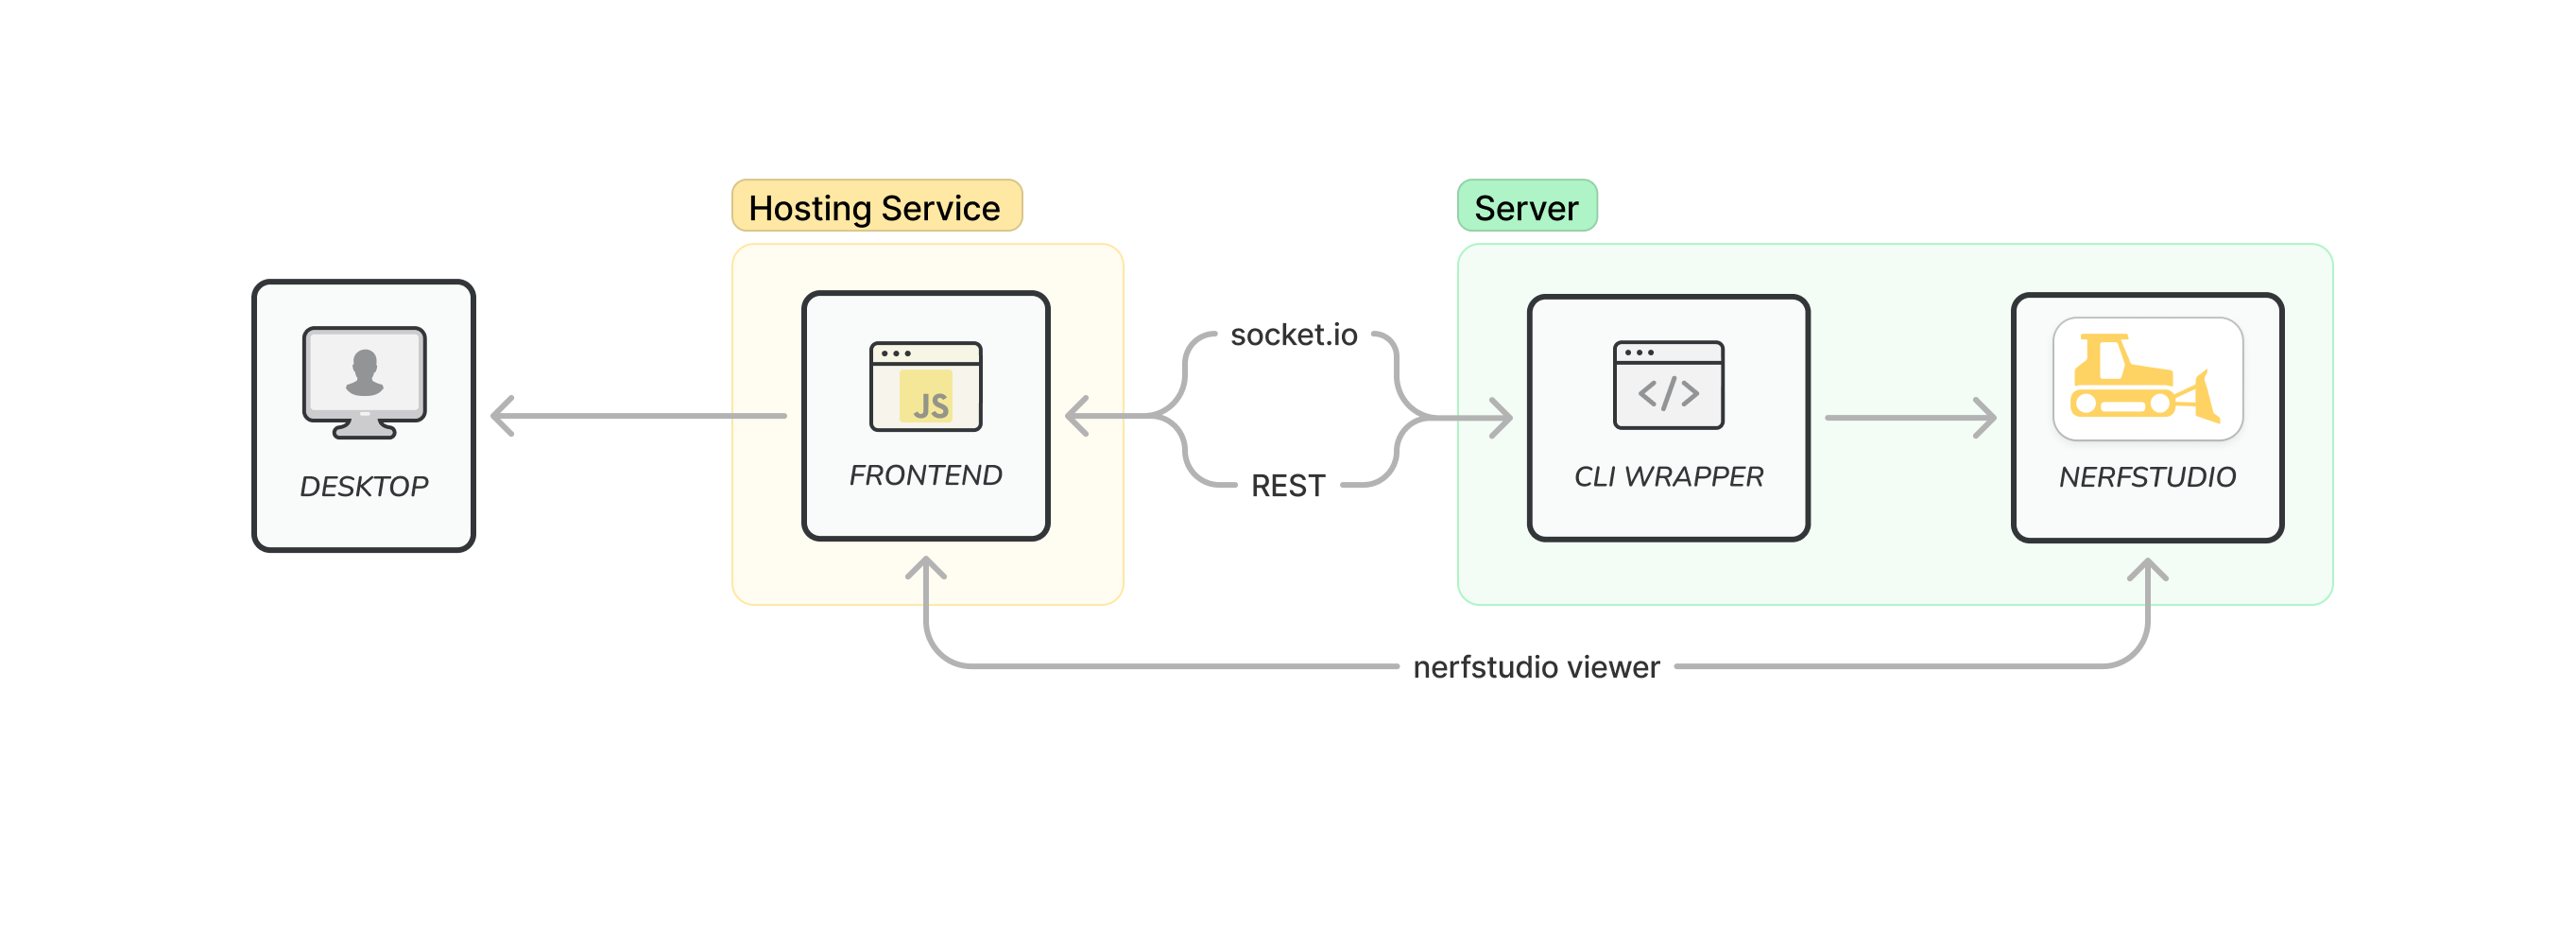
\includegraphics[width=\textwidth]{figures/architecture-1.png}
	\caption{System Architecture}
	\label{fig:system:example2}
\end{figure}

For the prototype, all the components were composed into a single docker container and deployed as a single unit.
This leveraged the pre-configured container provided by nerfstudio, and allowed for a quick and easy deployment of the prototype.

\section{Frontend Development} 
\label{sec:system:frontend}

% Setup, configuration, and component architecture
% UI/UX design principles

The frontend was built with React, as it is a popular and well supported framework for building web applications.
Vite was used as a build tool, as it provides a fast and efficient development experience.
To accelerate the styling process, Tailwind CSS was used, it is a utility-first CSS framework that provides a set of pre-defined classes that can be used to style components.
In additional the daisyUI component library provided a set of pre-styled components that could be used to quickly build the UI.

\subsubsection{Extensibility}

Extensibility was a key considerations during the development of the frontend, as the underlying nerfstudio CLI is in itself extendable.
All parameters for processing and training a NeRF model are configurable using JSON or strongly typed TypeScript objects.

\begin{lstlisting}[caption=Parameter Option configuration]
const stepsPerSave: NumberInput = {
	name: "stepsPerSave",
	label: "Steps Per Save",
	tooltip: "Number of steps between each save of the model.",
	inputType: "number",
	defaultValue: 1000,
};
\end{lstlisting}

Currently the supported input types are: number, select and boolean, but it is easy to add new types by extending the configuration object. 
It is also possible to define dependent parameters, that are only shown when a certain condition is met.
Images to illustrate the effect of a parameter can be added as well, to provide additional context to the user.

Filters and presets are also configurable using arrays of the names of the parameters that should be included in the filter or preset.
The full configuration can be found in the \texttt{frontend/src/config} folder in the codebase.

\subsubsection{Nerfstudio Viewer Integration}

The nerfstudio viewer is built using Viser, a library for building 3D visualizations using python.
This posed some limitations in integrating it into the frontend, as it is not easily possible to directly embed a python application into a web application.
To work around this, the viewer was hosted by nerfstudio as usual and embedded into the frontend using an iframe.

Some modifications could be made to the viewer to make it more suitable for embedding.
This included some simple styling changes to make the viewer fit better into the frontend.
The viewer contained several interactions where it was necessary for the user to copy console commands, to be used in the CLI.
These interactions were replaced with buttons that send a request to the server to execute the command instead.

These modifications were done at build-time of the container by applying a patch to the nerfstudio source code of the base image.


\section{Backend Development}
\label{sec:system:backend}

% Advantages of tRPC, configuration, and API design

The backend was built using tRPC, a framework for building type-safe APIs in TypeScript.
This type-safety was useful in building the API, as nerfstudio endpoints require a specific set of parameters of various types, that could be easily defined using TypeScript and reused in the frontend.

With tRPC, 

\section{Challenges and Solutions}
\label{sec:system:challenges}


\section{Lessons Learned}
\label{sec:system:lessons}

\section{Future Directions}
\label{sec:system:future}
         % INCLUDE: system
% !TEX root = ../main.tex
%
\chapter{Results}
\label{sec:result}


\section{Analysis of User Experience Questionaire}
\label{sec:result:ux}


\section{Findings from Qualitative User Testing}
\label{sec:result:testing}


\section{Integration and Findings}
\label{sec:result:findings}

         % INCLUDE: system
% !TEX root = ../main.tex
%
\chapter{Conclusion}
\label{sec:conclusion}
% TODO: Write conclusion

\section{Key Findings}
\label{sec:conclusion:findings}

\section{Contributions to the Field}
\label{sec:conclusion:contributions}

\section{Future Work}
\label{sec:conclusion:future}

     % INCLUDE: conclusion

% --------------------------
% Back matter
% --------------------------
\appendix\cleardoublepage
% !TEX root = ../main.tex
%
\chapter{Example Appendix}
\label{sec:appendix}

\Blindtext[1][1]

\section{Appendix Section 1}
\label{sec:appendix:sec1}

\Blindtext[1][1]

\begin{table}[h]
	\begin{tabularx}{\textwidth}{X | X | X}
		%\hline
		Alpha		& Beta			& Gamma			\\ \hline
		0			& 1				& 2				\\ \hline
		3			& 4				& 5				\\ %\hline
	\end{tabularx}
	\label{tab:table1}
	\caption{This is a caption text.}
\end{table}

\section{Appendix Section 2}
\label{sec:appendix:sec2}

\Blindtext[1][1]

\begin{table}[h]
	\begin{tabularx}{\textwidth}{X | X | X}
		%\hline
		Alpha		& Beta			& Gamma			\\ \hline
		0			& 1				& 2				\\ \hline
		3			& 4				& 5				\\ %\hline
	\end{tabularx}
	\label{tab:table2}
	\caption{This is a caption text.}
\end{table}

\Blindtext[1][2]
       % INCLUDE: appendix
%
{%
\setstretch{1.1}
\renewcommand{\bibfont}{\normalfont\small}
\setlength{\biblabelsep}{0pt}
\setlength{\bibitemsep}{0.5\baselineskip plus 0.5\baselineskip}
\printbibliography[nottype=online]
\newrefcontext[labelprefix={@}]
\printbibliography[heading=subbibliography,title={Webpages},type=online]
}
\cleardoublepage

\listoffigures
\cleardoublepage

\listoftables
\cleardoublepage

% !TEX root = ../main.tex
%
\pagestyle{empty}
\hfill
\vfill
\pdfbookmark[0]{Colophon}{Colophon}
\section*{Colophon}

This thesis was typeset with \LaTeXe.
It uses the \textit{Clean Thesis} style developed by Ricardo Langner.
The design of the \textit{Clean Thesis} style is inspired by user guide documents from Apple Inc.

Download the \textit{Clean Thesis} style at \url{http://cleanthesis.der-ric.de/}.

\cleardoublepage

\newpage
\mbox{}

% **************************************************
% End of Document CONTENT
% **************************************************
\end{document}
